\chapter{Design and Implementation}
While working on this project, I used the agile development, because the design and implementations of embedded devices such as the fingerprint and RFID is uncertain. I initially wanted to use a desktop application because 

Why NodeJS?

Why python?
python has a library for the fingerprint module(R3) I used. It also had a library for the raspberry pi(RC522) and how easy it is to write and test code.

Interfaces?
 research

An RFID is much more preferred because it identify tags without direct line of sight in contrast with the Barcodes, It is faster compared to other tracking methods 

\section{Approach}

I decided to go with Full Stack development, to understand and solidify my background in the fundamentals of web development. I decided to use an adaptation of the MERN stack which replaces the MongoDB with Azure to have a relational database.

\newacronym{MERN}{$MERN$}{MongoDB, Express, ReactJS, NodeJS}
\glsadd{MERN}
I divided this system into components 
I went with a website because it's easy to access from anywhere that has an internet connection and each part of the system can access each other cause they are all connected to the internet. I first thought about the languages and frameworks I would like to use. For the website (React), the web server (Node), and RFID and Fingerprint (Python). After that, I took into account the specification of the project; the software design process,

\subsection{Website - ReactJS}
Why ReactJS?
I started with wireframe diagrams and pictures of each pages and their functions, All the pages have a dashboard that acts as a navigation bar to get to different web pages. 

\subsubsection{Main page}
\begin{figure}[ht!]
  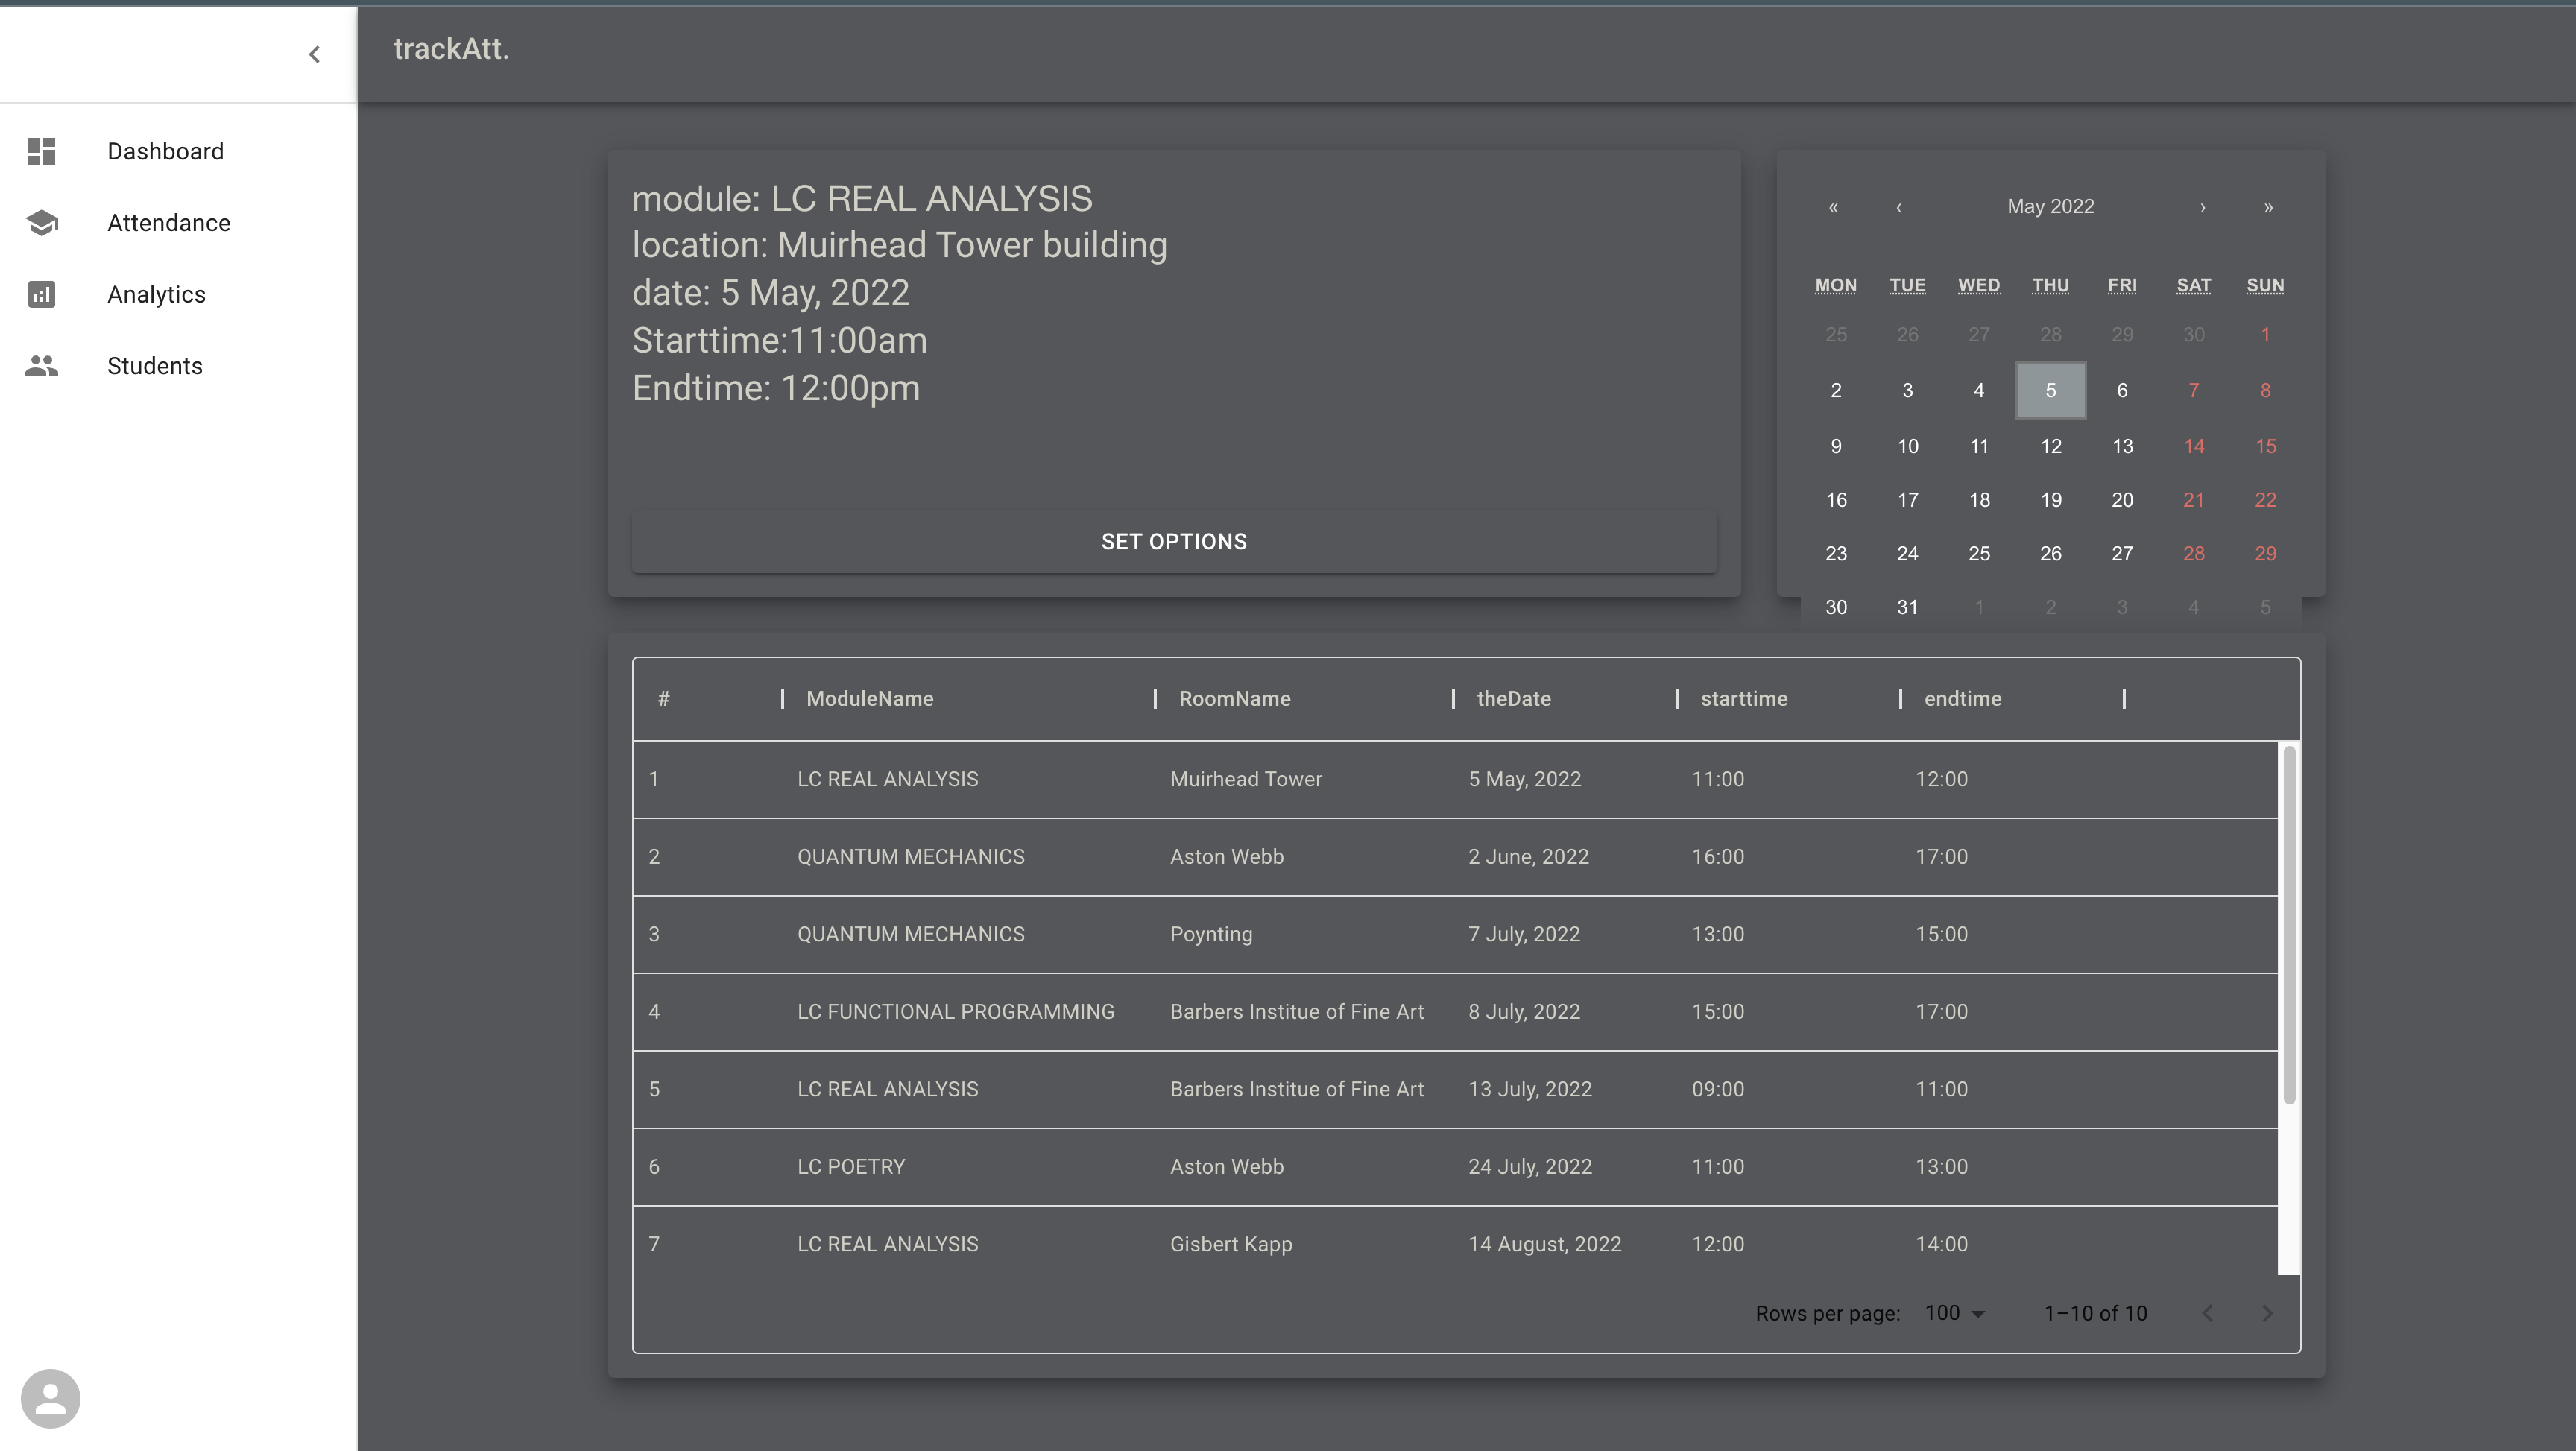
\includegraphics[scale=0.135]{Design & Implementation/images/Dashboard.png}
  \caption{Dashboard/Main page.}
\end{figure}
The main page consists of the EventView at the top left, the CalendarView at the top right and the EventList at the bottom.The functions of these views are:
\begin{itemize}
  \item CalendarView: A date picker that selects the date and sends a request to the server for an event on that date. The default date is the current date at that moment.
  \item EventView: it displays an events information if there is an event on the date requested by the Calendar. It also has a "Set options" button that allows the administrator/lecturer to choose tracking methods and options by redirecting to the Attendance page. 
  \item EventList: it displays a list of future events that the lecturer has.
\end{itemize}
Clicking the "trackAtt." header takes you to the main page.

\subsubsection{Attendance page}
\begin{figure}[ht!]
  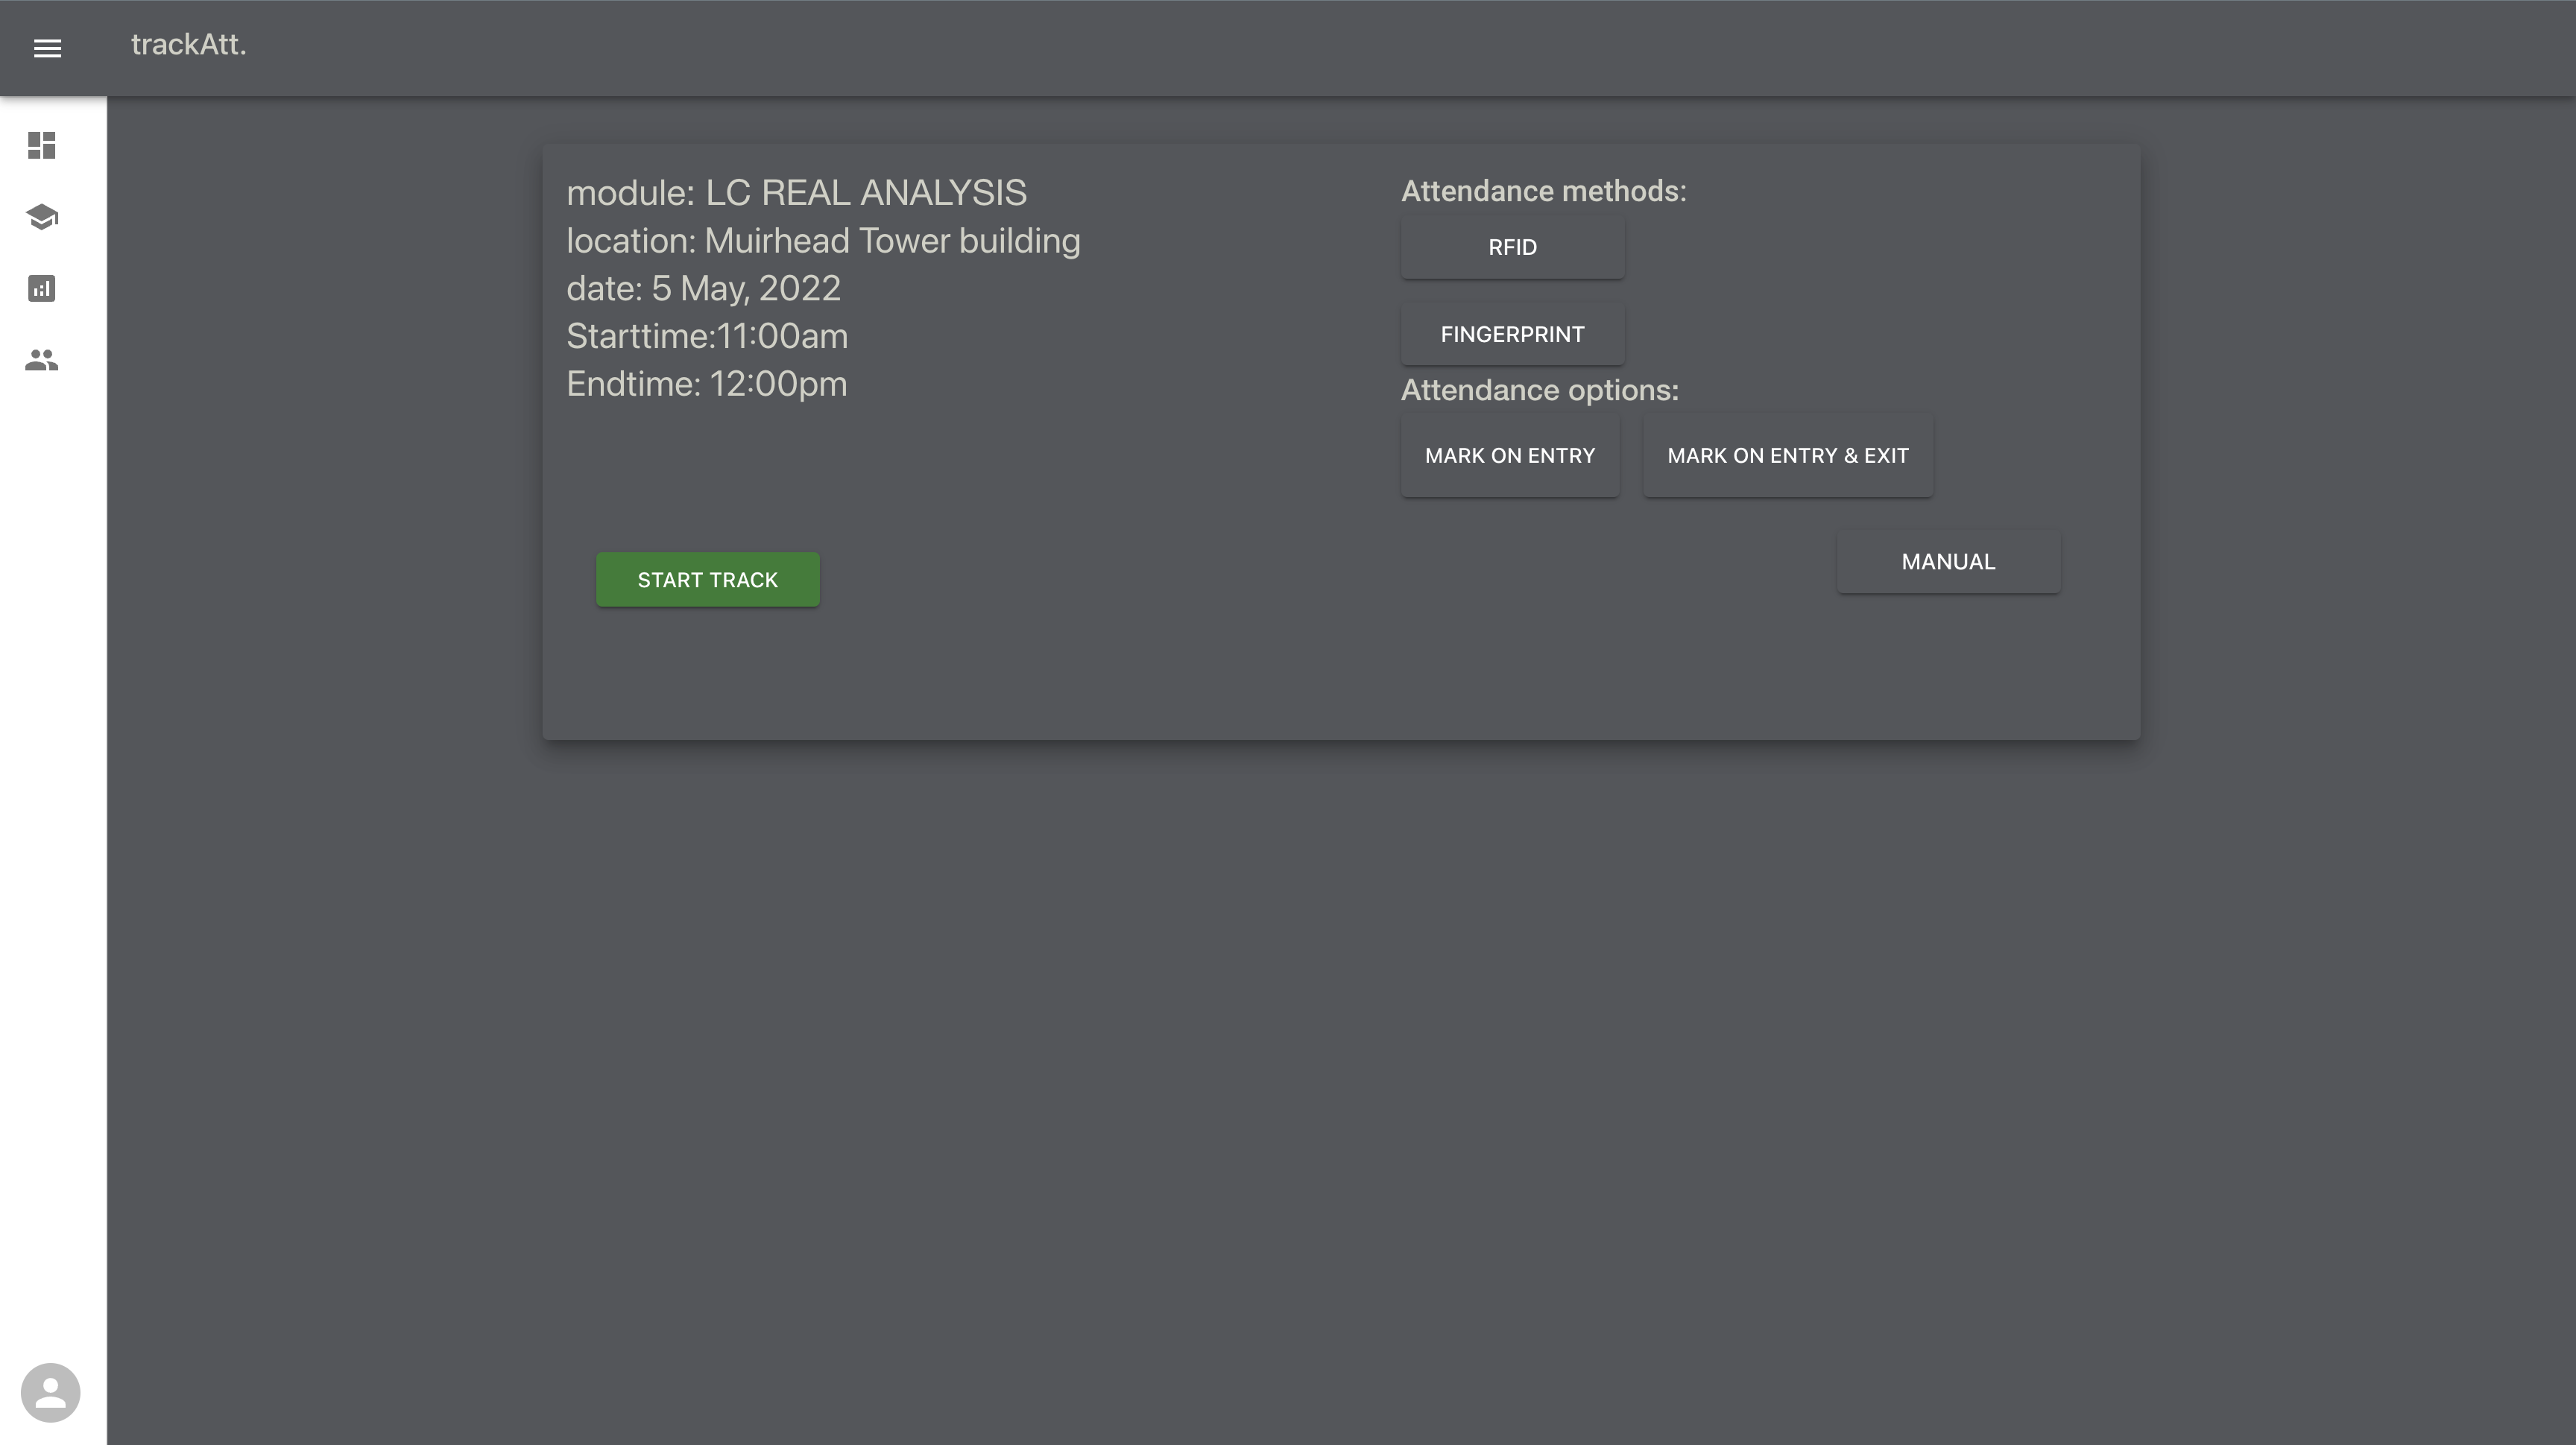
\includegraphics[scale=0.135]{Design & Implementation/images/Attendance.png}
  \caption{Attendance page.}
\end{figure}
The attendance page is mainly gotten to by the "Set options" button of the EventView, if directed to by the dashboard, it should show a list of events to track based on a picker. I couldn't develop this due to time. The main components of the Attendance page are the EventView but without a set options button. Attendance methods with RFID and fingerprint buttons, Attendance options with "mark only Entry" and "mark both Entry and Exit", a "Manual" button and a "Start Track" button. The functions of these components are;

\begin{itemize}
  \item EventView: displays information on the Event requested before by the CalendarView, gets a JSON response from the server and formats the 
  \item Attendance Methods: One method is chosen here, Either the Fingerprint method, the RFID method or the Manual method. Clicking on the fingerprint button sets the JM-101 module as the chosen method for tracking attendance while, clicking on the RFID button sets the RC522 module as the chosen method for tracking attendance, the manual method is for a worst-case scenario where the Raspberry-pi can not track attendance and the teacher knowing each students by name can tick who is absent or present, clicking the button redirects to the Manual page. 
  \item Attendance Options: just like the Attendance Methods just one option can be used, clicking the "mark on entry" button sets the chosen tracking method to track only when the user scans at the beginning of the event while, "mark on both entry \& exit" requires the user to scan at the beginning and end of the event.
  \item Start Track button: starts the tracking method with the attendance options chosen and also redirects to the "InProgress" page.  
\end{itemize}

\newacronym{JSON}{$JSON$}{JavaScript Object Notation}
\glsadd{JSON}

\subsubsection{InProgress page}
The InProgress page comprises of a timer, a "Stop Track" button and a UserView that shows a list of Students that are required for that module. initially I thought of displaying a list that refreshes every minute but did not because I thought this would be quite distractive to the admin while he's using the system for a different action. 


\subsubsection{Analytics page}
The Analytics page contains the Attendance status of the event that was tracked and a pie chart diagram that shows the percentage of student who attended that session. 

\subsubsection{Students page}
The Students page contains the whole list of students in the database.

\subsubsection{Manual page}
The Manual page displays a list of students each row has a checkbox that can be checked, If checked and submitted the students checked will be registered as present.



\subsection{Web server - NodeJS}
NodeJS is really good at handling simultaneous connections. In this project we're sending and receiving data from the database, the flask server and the front-end and sometimes they are concurrently. Tedious is a package that allows the implementation of TDS which is a protocol used to interact with SQL server, this allows me interact with the azure database.
The reason express is used in my project is to mount a middleware at the router-level, this allows me to handle multiple request and responses to multiple end-points with one single mounted root path. 

using the mvc architecture for developing the backend the controller attendanceController.js handles the logic of
These are the major requests and responses handled by the express middleware;
\begin{itemize}
    \item receiveDate: a POST request that sets the date received from the client
    \item sendEvent: a GET request that runs a query to the database that gets all details of an event on a specific date and sends a \gls{JSON} response to the client
    \item sendEventList: a GET request that queries the database that for a list of events which is sent to the client and displayed on the EventList
    \item startTrack: a POST request that gets an Object that consists of the tracking method and option chosen and sends a POST request to the Flask server that runs a script to that start the method chosen
    \item stopTrack: a POST request that checks the method running based on a glob§al variable that was initially set when startTrack was called and sends a POST request to the Flask server endpoint to stop the process
    \item showAttendanceList: a POST request that queries the database for students taking a module based on a classID value that's already been set for the current Event, this returns a response that sends a table containing who was present and absent(status)
    \item showAttendanceListWithoutStatus: a GET request that returns students taking a module based on a classID value
    \item showStudentList: a GET request that returns a list of students taking the current module that is being tracked
    \item showManualAttlist: a GET request similar to the showStudentList but the response is formatted in the front-end
    \item calculateAttendance: a GET request that returns the number of students who are present and absent, this sent to the front-end makes up the pie-chart
    \item addToAttManually: a POST request that adds users from an array gotten from the front-end.
\end{itemize}



\newacronym{TDS}{$TDS$}{Tabular Data Stream}
\glsadd{TDS}
\subsection{Raspberry pi}
I focused on writing a script for the RFID to read information from the RFID tags, when I finished that, I wrote a script to 
I researched on python libraries for RFID
At first I wanted to call each python scripts from the web server but I ran into a series of errors coming from Raspberry pi not being able to grant access for that, and then I found out how to use flask and I came up with the idea of running these scripts from a http endpoint of the flask server.
\subsubsection{fingerprint}
The python Library used was 
At first I was thinking of 

\subsection{Flask}
A major reason why I chose to use flask is because it creates a local server in python, so I don't have to run python scripts in a different language or use an external framework for this.
These are the major requests and responses handled by the flask functions and endpoint.



\subsection{Database}
The database was difficult and complex because of the relationships between different tables, I spent 60\% of my time updating it to fit other parts of the project. I needed it to be hosted on the internet to access it on multiple devices, raspberry and my development computer, At first I used a local MySQL database on my computer but had an issue hosting this on the internet, I switched to Azure because it offered a lot more of other cloud computing services. I created the student table with:

\begin{figure}[ht]
  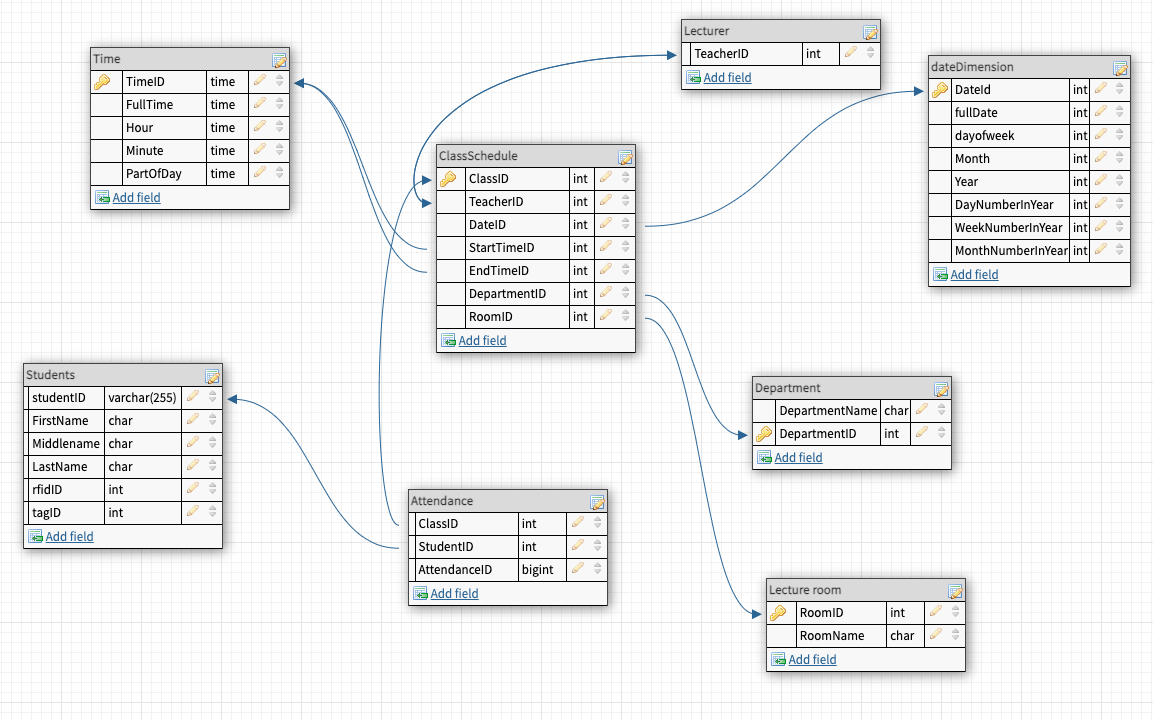
\includegraphics[scale=0.4]{Design & Implementation/images/database_design.png}
  \caption{database design}
\end{figure}
